\section{Methods}
\label{sec:methods}
In response to stakeholder and public wants, forest planners often manage forests for multiple ecosystem services simultaneously, such as wildlife habitat, recreation, goods production, aesthetics, and carbon sequestration. Such ecosystem services are commonly in conflict with one another, meaning that forest planners cannot simultaneously maximize the provision of all ecosystem services. Instead, provision of some services must be sacrificed to enable achievement in others, forcing the forest planner to seek a best compromise among the bundle of ecosystem services.

It is currently unknown how climate change will alter the tradeoff relationships among bundled ecosystem services. This drives uncertainty in how forest planners may have to change their compromise strategies to maintain a desired balance among ecosystem services. In this section, I describe a case study in the Deschutes National Forest to quantify the changes in tradeoff relationships and how understanding these changes may result in better management decisions. To quantify the changes in the tradeoff relationships, I employ multi-objective mathematical optimization and compare the results under three different climate change scenarios.

\subsection{Study system}
\label{subsec:studyArea}
The Drink Planning Area is a 7056 ha area on the east slopes of the Cascade Mountain Range in the Deschutes National Forest (see Figure \ref{fig:drinkOverview}). Like many managed forests, the Drink is managed for the simultaneous provision of multiple ecosystem services.  The managing entity, the US Forest Service, has specified a bundle of three ecosystem services for prioritization.

\begin{figure}[ht]
\centering
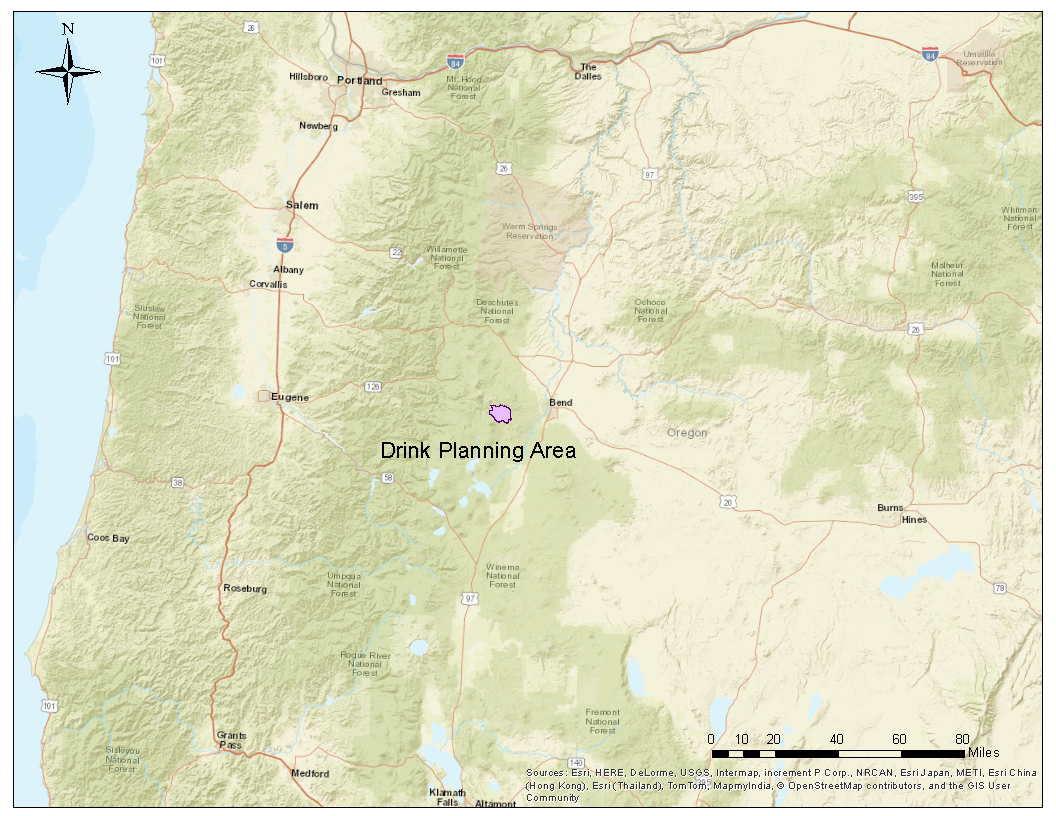
\includegraphics[width=.85\textwidth]{../images/DrinkMap_Overview}
\caption[Overview of the study system, the Drink Planning Area]{Overview of the study system, the Drink Planning Area (in purple), consisting of 7056 ha in the Deschutes National Forest.}
\label{fig:drinkOverview}
\end{figure}

The first ecosystem service is the provision of habitat for the northern spotted owl (NSO) (\textit{Strix occidentalis caurina}). The NSO is a common, if controversial, indicator species in Pacific Northwest forests. Because of the availability of dense old growth forest in the Drink, approximately 43\% of the area serves as habitat for the NSO (see Figure \ref{fig:drinkOwlAndWatershed}). The USFS is required to protect this species since it is listed as threatened and therefore protected by the Endangered Species Act of 1973 \cite{congress1973endangered}.

The second ecosystem service the USFS seeks to provide is protection from wildfire. This protection is achieved by way of silvicultural treatments applied to designated treatment areas (stands) across the Drink. The efficacy of these treatments is measured by comparing the fire hazard rating of the stand before and after treatment. The fire hazard rating is described in more detail below and in table \ref{tab:firehazards}. Implementing the silvicultural treatments to reduce the fire hazard rating of the Drink is critical not only because it protects the habitat of the NSO, but also because the Drink Area houses the municipal watershed for the cities of Bend, OR and Sisters, OR (see Figure \ref{fig:drinkOwlAndWatershed}). Wildfires pose a threat to these cities' water supply, because wildfires can cause soil water repellency, surface runoff, and debris torrents \cite{ice2004effects}. In addition, the Drink has never before undergone fuels treatments, which increases the expected severity of a fire should one occur. 

\begin{figure}
\centering
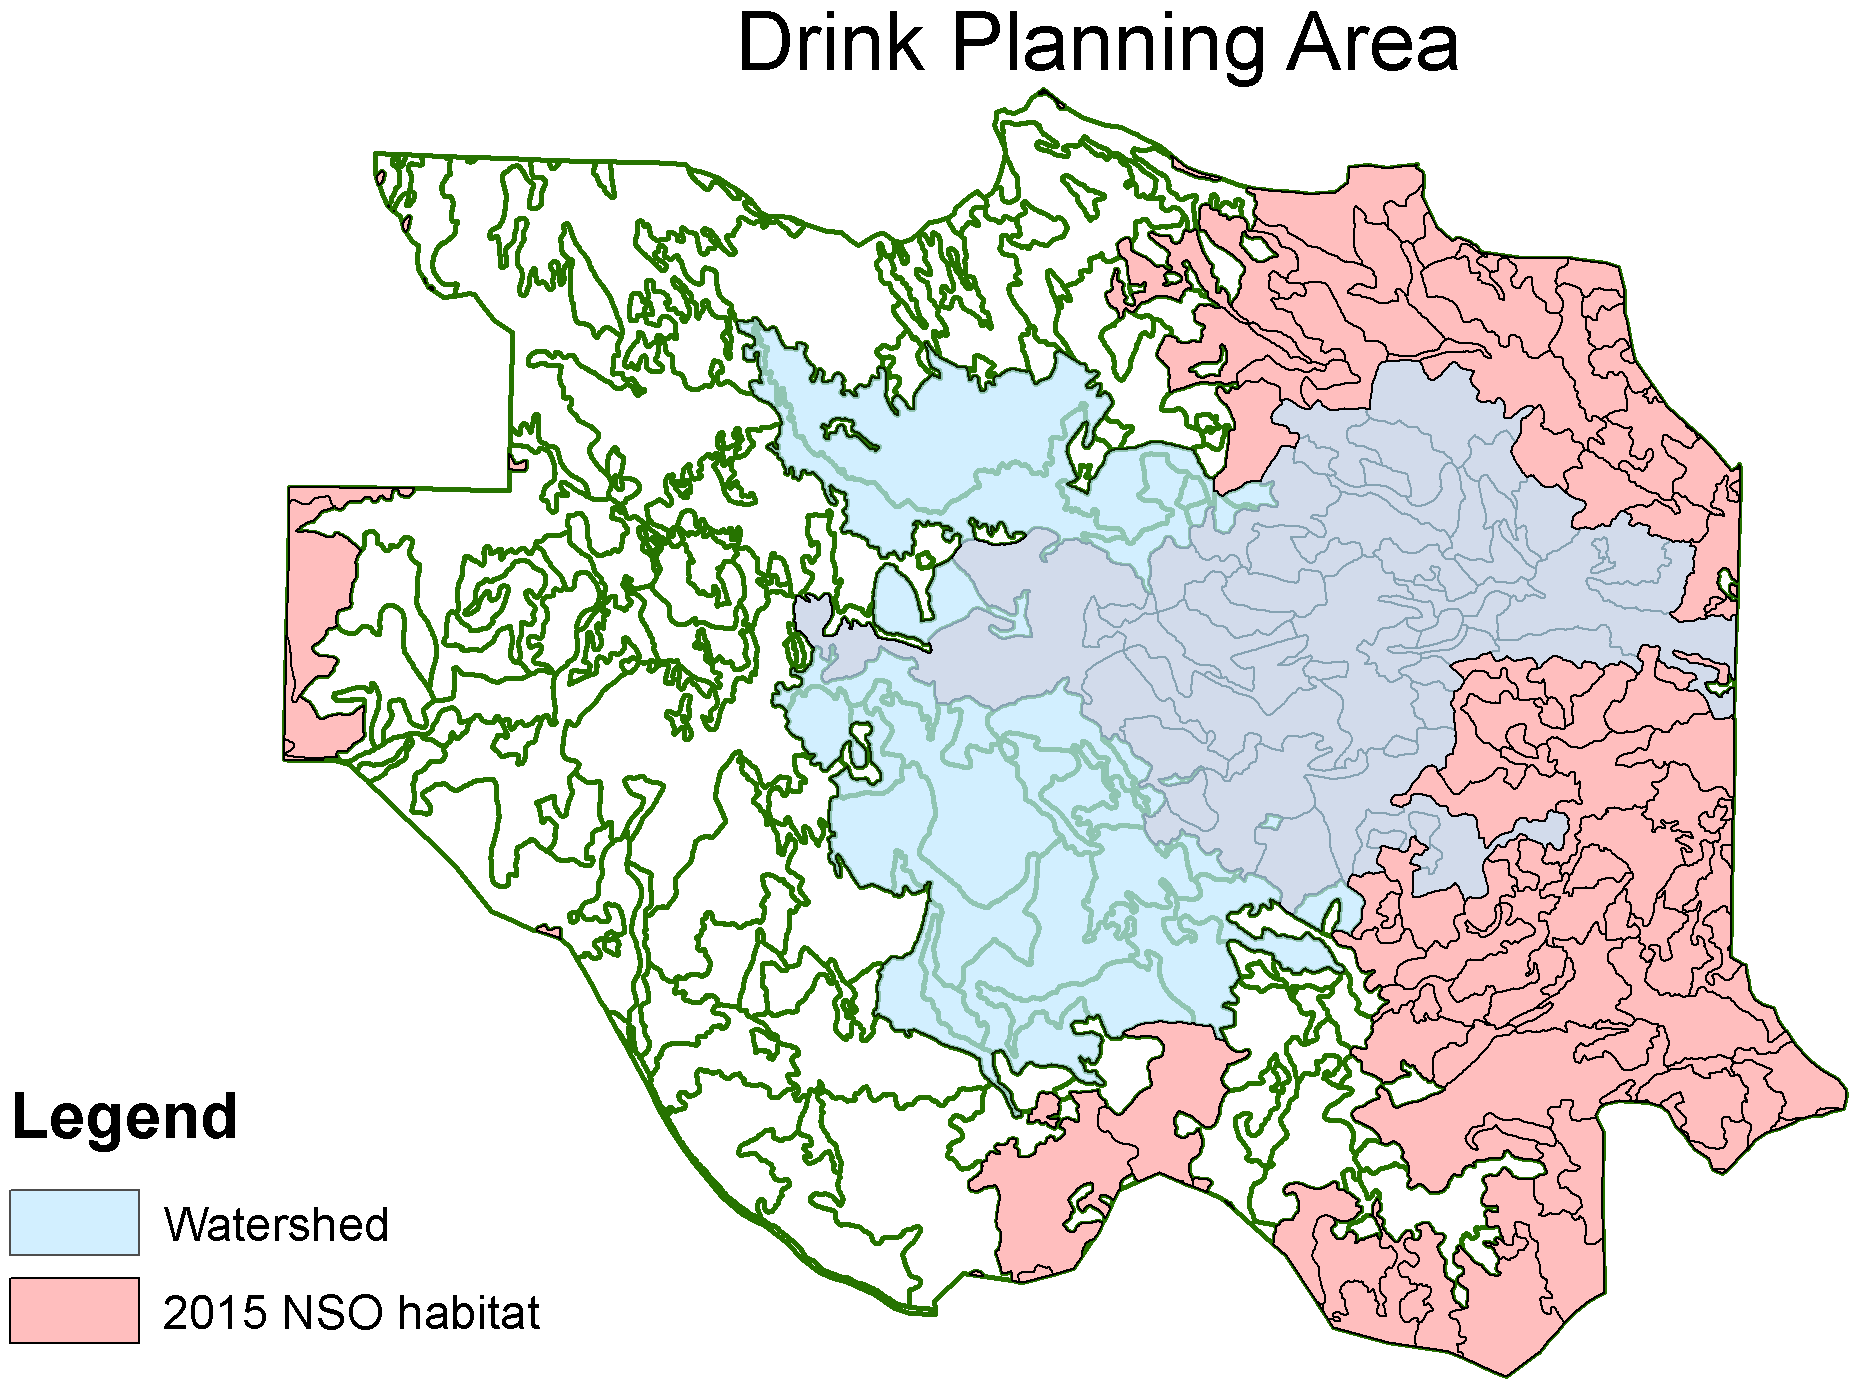
\includegraphics[width=.5\textwidth]{../images/DrinkMap_NSOAndWatershed}
\caption[NSO Habitat and municipal watershed in the Drink Planning Area]{Location of the municipal watershed and the suitable NSO habitat in the Drink area at the beginning of the planning horizon (2015). Interior polygons are the 303 management units.}
\label{fig:drinkOwlAndWatershed}
\end{figure}

The last ecosystem service is the provision of a watershed with minimal sediment content. While the silvicultural treatments intend to provide long-term protection of the watershed, the implementation of the treatments has the potential to introduce short-term increases in sediment delivery to the watershed \cite{o2005conceptual}. This is expected to be especially true in the Drink Area, where local Forest Service staff have noted that the watershed is unusually susceptible to spikes in sediment delivery as a result from activities within the watershed.

\subsection{Timeline and assessment of treatment efficacy}

This study of the Drink Planning Area consists of an 80 year planning horizon (2015 - 2095). All silvicultural treatments will be scheduled for application in the first 40 years (2015 - 2055), divided into two 20-year planning periods (2015-2035 and 2035-2055). Spatially, the Drink is divided into 303 forest stands. Each stand may be assigned a treatment in either period, in neither period, or in both periods. Determining which treatment type to apply to a stand was done \textit{a priori} and is entirely dependent on silvicultural characteristics; the rules governing this assignment of treatment type can be found in the appendix, \S \ref{chap:appBTreatmentSpec}.

\begin{figure}
\centering
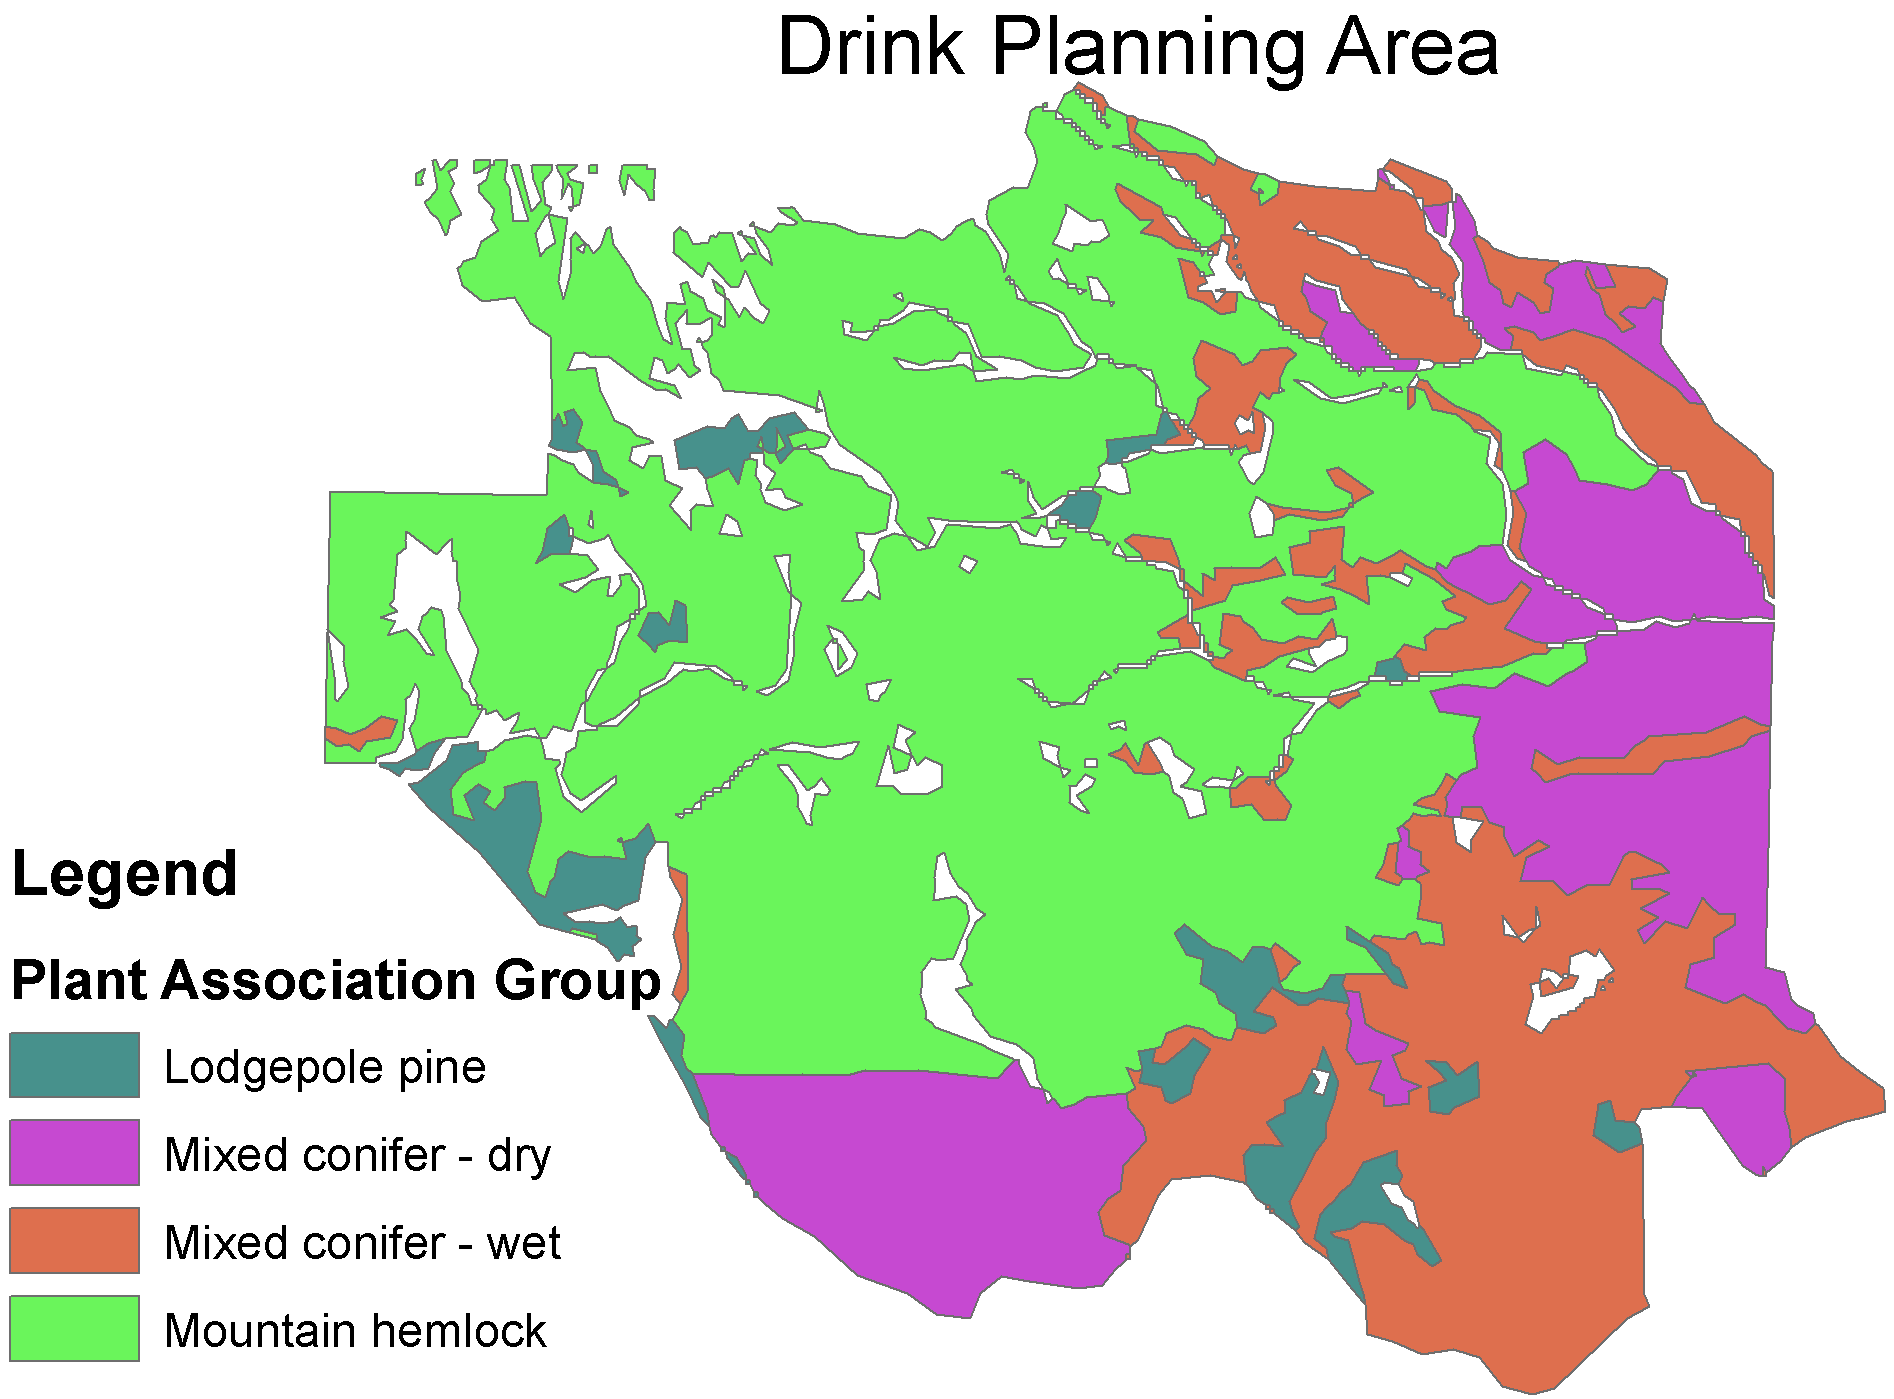
\includegraphics[width=.5\textwidth]{../images/DrinkMap_PAGs}
\caption[Plant association groups in the Drink Planning Area]{Plant association groups in the Drink Planning Area that were selected for potential treatments. Other plant association groups exist in the area but were not considered for treatment.}
\label{fig:drinkPAGs}
\end{figure}

To assess the treatments' long-term efficacy, the fire hazard rating of the Drink is measured at the end of the 80-year planning horizon in year 2095. The area of NSO habitat is assessed at the end of each planning period, years 2035 and 2055, to ensure that the application of treatments does not negatively impact the available habitat. Finally, the resulting short-term spikes in sediment delivery are measured at the time of treatment.

The time of treatment is assumed to be at the midpoint year in the planning period, years 2025 and 2045. A schematic of the planning horizon including the time of these events is shown in Figure \ref{fig:drinkPlanningHorizon}.

\begin{figure}
\centering
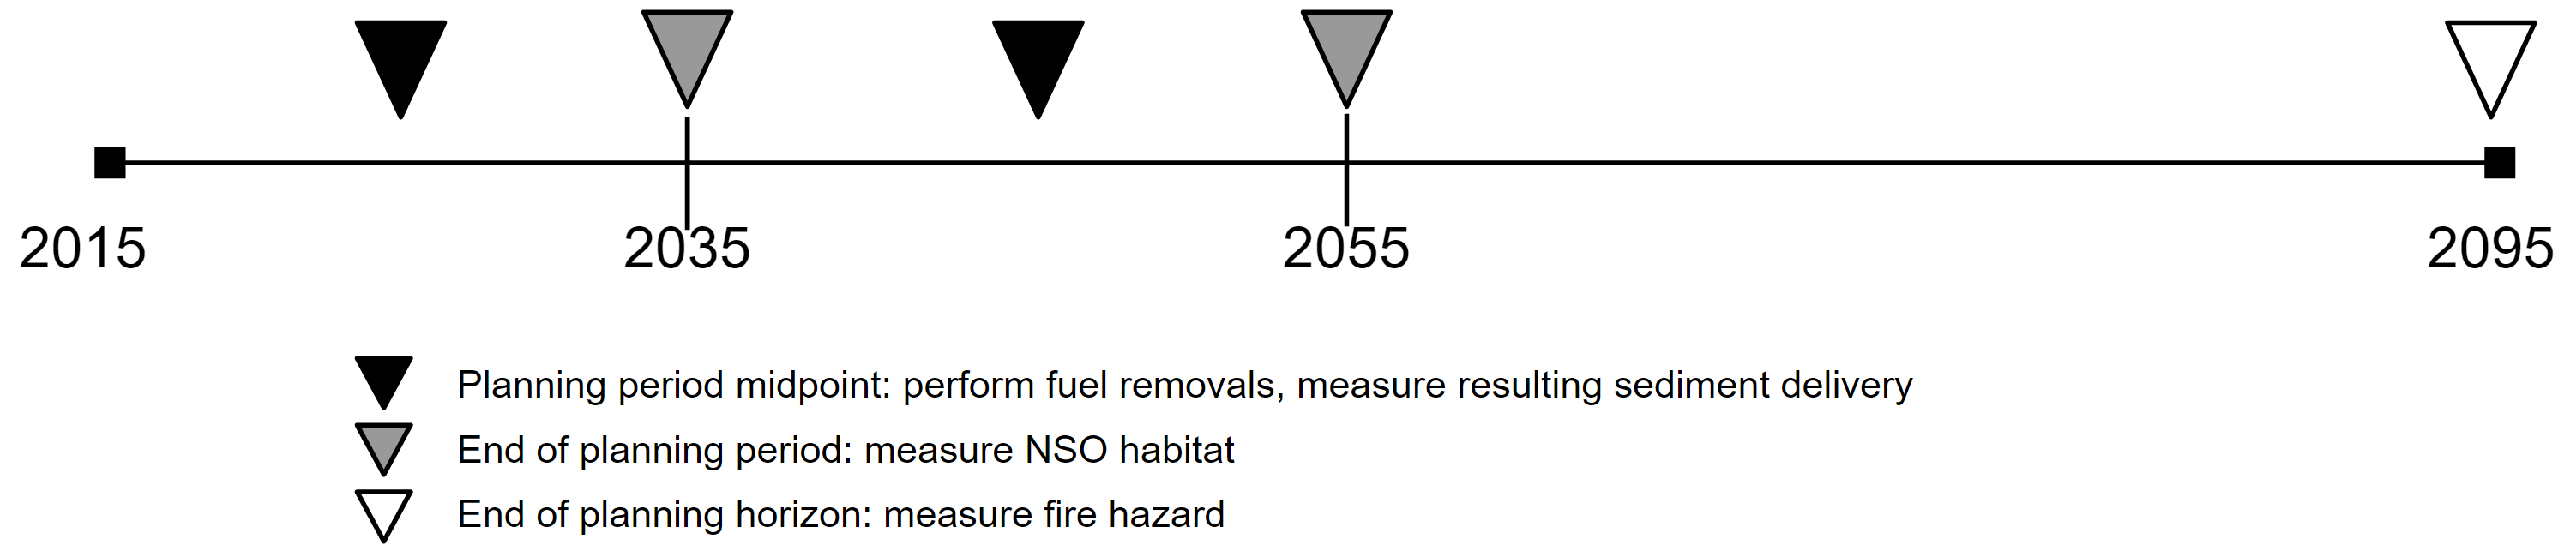
\includegraphics[width=.85\textwidth]{../images/Drink_PlanningHorizon_Sketch}
\caption[Planning horizon schematic]{The planning horizon used in the analysis spans the 80 year period from 2015 to 2095. Treatments may be performed in the first period, the second period, both, or neither. Treatments are assumed to be performed at the mid-point years of each period (black triangles). Sediment delivery is measured on treatment years. Stands' suitability for NSO habitat is measured at the end of the planning periods (gray triangles), and stands' fire hazard ratings are measured at the end of the planning horizon (white triangle).}
\label{fig:drinkPlanningHorizon}
\end{figure}

There is competition among the bundled ecosystem services: fuel treatments in the watershed drive short-term peaks in sediment delivery and have the potential to reduce owl habitat, yet the prioritization of either NSO habitat or water quality alone entails fewer fuel treatments and increased fire hazard rating as a result. The USFS seeks a management plan that balances the provision of these bundled ecosystem services. The ability of the forest planner to decide on such a plan may be improved given a better understanding of the tradeoff relationships among the ecosystem services in the bundle. In this study, I address the novel question of how climate change impacts these tradeoff relationships.

\subsection{Climate Scenarios Considered}
In their assessments on the changing climate, the IPCC uses a scenario-based approach, presenting many models of future climates from research agencies around the world. There is no attempt to predict which of the future climates is most likely or quantify the probability of realization of any one scenario. The same approach is employed here in studying the potential impacts of climate change on tradeoff relationships among bundled ecosystem services.

In this work, the alternative future climates considered are climate scenarios from the first working group (WG1) of the IPCC's Fifth Assessment (AR5) \cite{ipcc2013climate}. Given the large number of potential future climates considered by the IPCC (see the list of experiments considered in AR5 \cite{ipccListOfAR5Models}) combined with the computational complexity involved in the study of each one, I selected a small subset of three future climate scenarios for this analysis. Hereafter the scenarios are referred to as ``None'', ``Ensemble RCP 4.5'', and ``Ensemble RCP 8.5''.

The first scenario, ``None'', is the assumption of no climate change. While the number of studies incorporating climate change is increasing, this is still the assumption used for many modern studies such as Schroder (2013) \cite{schroder2016multi}, from which this study is derived. Because it has served as the basis for many studies and assumes a static environment resembling today's, the ``None'' climate scenario serves as a good control against which to compare the other two future climate scenarios.

As their names suggest, the second and third scenarios are ensembles. Each ensemble is an assembly of 17 global circulation models (GCMs) used in IPCC AR5. The selection of component GCMs in the ensembles was performed by the USFS's Climate-FVS \cite{dixon2002essential} team. The list of the 17 scenarios included in the ensemble can be found in Crookston (2016) \cite{ClimateModelsInFVSEnsemble}. Each component GCM has a corresponding climate surface which contains a vector of 35 climate parameters at over 11,000 global locations for three time periods. The climate surfaces for the ensembles were created by averaging the values of all component GCMs for each climate parameter and each time period for each location. The result is a climate surface that, while temporally sparse, is spatially robust. Such a configuration is suited for use in the Drink area given the area's variance in elevation and slow vegetation growth.

The two ensembles are comprised of the same 17 GCMs, but the assumed representative concentration pathways (RCP) in the component GCMs differ. The RCP indicates the additional radiative forcing in $W/m^2$ above pre-industrial levels, with higher values of forcing indicative of more severe climate change. The GCMs in the Ensemble RCP 4.5 scenario assume 4.5 $W/m^2$ of additional radiative forcing, and the GCMs in the Ensemble RCP 8.5 scenario assume 8.5 $W/m^2$ of additional radiative forcing.

These three scenarios were chosen for the analysis because they represent a range of predicted climate change severity, from a $0 \degree C$ warming by the year 2100 under the ``None'' scenario to a $2.6-4.8 \degree C$ warming under RCP 8.5 \cite{ipcc2013climate}.

\subsection{Determining tradeoff relationships between ecosystem services and climate scenarios}
\label{subsec:whyUsingMultiObjModel}
Each climate scenario is used to parameterize a multi-objective mathematical optimization model. These models determine the allocation of resources for optimal achievement of the objectives. Here, the resources are the application of fuel treatments and the objectives are the ecosystem services prioritized by the Forest Service: NSO habitat, fire hazard reduction, and short-term sediment delivery.

Solving each model generates a suite of management alternatives providing varying amounts of each ecosystem service. Comparing the ecosystem service achievements across the management alternatives reveals the tradeoff relationships among the ecosystem services. Since each model is parameterized according to a particular climate scenario, comparing the tradeoff relationships across models reveals how climate change impacts these tradeoffs among ecosystem services.

\subsection{The Multi-objective Optimization Model}
\label{sec:model}
This section describes the multi-objective zero-one mathematical program to optimize the joint provision of ecosystem services in the Drink area. The model minimizes the fire hazard rating of the area, minimizes the peak sediment delivery occurring as a result of performing fuel treatments, and maximizes the minimum area of NSO habitat after treatment periods in the planning horizon.

\subsubsection{Notation}
The following notation is used throughout the model:
\paragraph{Parameters}
\begin{itemize}
\item \textbf{$i \in I$:} the set of all 303 stands in the Drink area
\item \textbf{$r \in R$:} the set of treatment schedule prescriptions:
	$$
	r =
	\begin{cases}
	1 &\text{ treatment applied in the first period (2015-2035)}\\
	2 &\text{ treatment applied in the second period (2035-2055)}\\
	3 &\text{ treatment applied in both periods}\\
	0 &\text{ no treatment applied in either period}
	\end{cases}
	$$
\item \textbf{$F_{i,r}$:} the area-weighted fire hazard rating of stand $i$ at the end of the planning horizon if prescribed to treatment schedule $r$
\item \textbf{$I_{\omega,t}$:} the set of stands that can qualify as NSO habitat at the end of planning period $t$
\item \textbf{$a_i$:} the area of stand $i$
\item \textbf{$e$:} the discount factor applied to NSO habitat that is less than 200 ha in size
\item \textbf{$j \in R_{i,t}$:} the set of treatment schedules such that stand $i$ qualifies as NSO habitat in planning period $t$
\item \textbf{$s_{i,t}$:} the contribution in tons of sediment delivered from performing fuel treatments on stand $i$ in planning period $t$
\item \textbf{$c \in C$:} the set of all clusters of stands whose combined area exceeds 200 hectares
\item \textbf{$i \in D_c$:} the set of all stands that comprise cluster $c$
\item \textbf{$c \in C_i$:} the set of all clusters that contain stand $i$
\item \textbf{$A$:} the maximum area in hectares that may be treated in either planning period
\item \textbf{$\ell$, $u$:} the lower and upper bounds, respectively, on the relative fluctuation in the area treated in periods 1 and 2
\end{itemize}

\paragraph{Decision Variables}
$$
x_{i,r} = \begin{cases}
1 &\text{ if stand $i$ is prescribed to treatment schedule $r$}\\
0 &\text{ otherwise}
\end{cases}
$$ 

\paragraph{Indicator Variables}
\begin{itemize}
\item \textbf{$q_{c,t} = 1$} if all stands in cluster $c$ qualify as NSO habitat in planning period $t$ and $q_{c,t} = 0$ otherwise
\item \textbf{$p_{i,t} = 1$} if in planning period $t$ stand $i$ is part of a cluster $c$ such that $q_{c,t} = 1$; $p_{i,t} = 0$ otherwise
\end{itemize}

\paragraph{Accounting Variables}
\begin{itemize}
\item \textbf{$S_t$:} the contribution in tons of sediment delivered from performing fuel treatments in planning period $t$
\item \textbf{$O_t$:} the amount of NSO habitat in hectares at the end of planning period $t$
\item \textbf{$H_t$:} the area in hectares treated in planning period $t$
\end{itemize}

\subsubsection{Parameterization}
The model was parameterized as follows:
\begin{itemize}
\item \textbf{$F_{i,r}$:} the metric for fire hazard rating used in this analysis originated in the work by Schroder \textit{et al.} \cite{schroder2016multi}. This metric was developed for the Drink area. It combines fire characteristics from Anderson's fuel models \cite{anderson1982aids} to assign a fire hazard rating. I expanded the rating system to include fuel models not present in Schroder \textit{et al.} See Table \ref{tab:firehazards}.

The stands' fuels and vegetation characteristics to determine the fire hazard rating were generated using the US Forest Service's Climate-Forest Vegetation Simulator (FVS). Input vegetation data to Climate-FVS came from the 2012 GNN structure map (\url{http://lemma.forestry.oregonstate.edu/data/structure-maps}) from Oregon State University's Landscape Ecology, Modeling, Mapping \& Analysis (LEMMA) group. Plots from the LEMMA database were mapped to the stands in the Drink area in order to produce tree and stand lists. These lists were used with Climate-FVS to simulate the stands' vegetation and fuels characteristics forward for the duration of the planning horizon under each climate scenario. Input climate data for Climate-FVS was obtained through the Climate-FVS climate data server \cite{climateFVSReadyData}.
\item \textbf{$I_{\omega,t}$:} the set of stands that qualify as NSO habitat at the end of a planning period $t$ are those that meet the following three criteria, as specified by the USFS:
	\begin{enumerate}
	\item elevation less than 1830 m
	\item the presence of trees with DBH no less than 76 cm
	\item canopy closure of at least 60\%
	\end{enumerate}
The elevation requirement was checked using a digital elevation model from the US Department of Agriculture's GeoSpatial Data Gateway; canopy closure and large tree requirements were determined using the simulated vegetation characteristics output from Climate-FVS.

To account for the NSO's large habitat requirements, stands must also be members of a cluster exceeding 200 ha in size, all of which meet the above three NSO habitat criteria. Stands not part of such a cluster have their contributions to owl habitat discounted by a factor of $e$.
\item \textbf{$e$:} the discount factor for sub-200 ha NSO habitat was set to $e = 0.5$ following the convention used in Schroder \textit{et al.} \cite{schroder2016multi}.
\item \textbf{$j \in R_{i,t}$:} each stand-treatment schedule combination is evaluated at the end of each planning period to determine its suitability as NSO habitat. Treatment schedules for which stand $i$ meets the criteria described above become members of the set $R_{i,t}$. 
\item \textbf{$s_{i,t}$:} the contributions of sediment delivery were determined using the Watershed Erosion Prediction Project (WEPP) online GIS tool \cite{frankenberger2011development}. This tool takes as input soil textures, treatment types, duration of simulation, and custom climate data. I obtained soil texture data for the Drink area from the USDA's Soil Survey Geographic (SSURGO) database. Treatment types are those specified in \S \ref{chap:appBTreatmentSpec}, and the years of simulation correspond to the treatment years in the model's planning horizon. The custom climate data are the same data described above for use with Climate-FVS, obtained through the Climate-FVS data server.
\item \textbf{$A$:} the maximum area that may be treated in either planning period was defined to be 6000 acres, or approximately 2428 ha
\item \textbf{$\ell$, $u$:} the relative fluctuation in the area treated in periods 1 and 2 was defined to be 20\%. That is, $\ell = 0.8$ and $u = 1.2$.
\end{itemize}
\begin{table}[!ht]
\centering
\resizebox{\textwidth}{!}{%
\begin{tabular}{l|c|crrr}
\multicolumn{1}{c|}{Fuel Model} & \multicolumn{1}{c|}{\textbf{Fire Hazard Rating}} & \multicolumn{1}{c}{Group} & \multicolumn{1}{c}{Flame length (m)} & \multicolumn{1}{c}{Rate of spread (m/hr)} & \multicolumn{1}{c}{Total fuel load (tons/ha)} \\ \hline
4*                              & \textbf{5}                                       & Shrub                     & 5.79                                 & 1508.76                                   & 32.12                                         \\
5                               & \textbf{4}                                       & Shrub                     & 1.22                                 & 362.10                                    & 8.65                                          \\
8                               & \textbf{1}                                       & Timber                    & 0.30                                 & 32.19                                     & 12.36                                         \\
9*                              & \textbf{2}                                       & Timber                    & 0.79                                 & 150.88                                    & 8.65                                          \\
10                              & \textbf{2}                                       & Timber                    & 1.46                                 & 158.92                                    & 29.65                                         \\
11*                             & \textbf{2}                                       & Logging Slash             & 1.07                                 & 120.7                                     & 28.42                                         \\
12                              & \textbf{4}                                       & Logging Slash             & 2.44                                 & 261.52                                    & 85.50                                         \\
13                              & \textbf{5}                                       & Logging Slash             & 3.20                                 & 271.58                                    & 143.57                                       
\end{tabular}%
}
\caption[Fire hazard ratings used in multi-objective model]{Fire hazard rating system used here, originally employed by Schroder \textit{et al.} \cite{schroder2016multi}.\\
* denotes fuel models not present in Schroder \textit{et al.}\\
The fuel model column refers to the Anderson fuel model ratings \cite{anderson1982aids}.}
\label{tab:firehazards}
\end{table}

\subsubsection{Formulation}
The formulation of the model is as follows:
\begin{align}
Minimize \quad & \notag\\
&\sum_{i\in I}\sum_{r\in R} F_{i,r} x_{i,r} \label{eqn:objFire} \\
&\max \{S_1,S_2\} \label{eqn:objSediment} \\
Maximize \quad & \notag\\
&\min \{O_1,O_2\} \label{eqn:objOwl}
\end{align}
Subject to:
\begin{align}
\sum_{i\in I_{\omega,t}} \left(a_i p_{i,t} + e a_i \left( \sum_{j \in R_{i,t}} x_{i,j}-p_{i,t} \right) \right) &= O_t \qquad \forall t \in \{1,2\} \label{eqn:constraintDefOwl}\\
\sum_{i\in I} \sum_{r\in 1,3} s_{i,1} x_{i,r} &= S_1 \label{eqn:constraintSediment1} \\
\sum_{i\in I} \sum_{r\in 2,3} s_{i,2} x_{i,r} &= S_2 \label{eqn:constraintSediment2} \\
\sum_{i \in D_c} \sum_{j \in R_{i,t}} x_{i,j} - |c| q_{c,t} &\ge 0 \qquad \forall t \in \{1,2\}, c \in C \label{eqn:constraintClusterTriggers} \\
\sum_{c \in C_i} q_{c,t} - p_{i,t} &\ge 0 \qquad \forall t \in \{1,2\}, i \in I_{\omega,t} \label{eqn:constraintPVarTriggers} \\
\sum_{r \in R} x_{i,r} &= 1  \qquad \forall i \in I \label{eqn:constraintOnePrescrip} \\
\sum_{i \in I} \sum_{r \in 1,3} a_i x_{i,r} &= H_1 \label{eqn:constraintAreaAcctg1} \\
\sum_{i \in I} \sum_{r \in 2,3} a_i x_{i,r} &= H_2 \label{eqn:constraintAreaAcctg2} \\
H_t &\le A \qquad \forall t \in \{1,2\} \label{eqn:constraintAreaRestr} \\
\ell H_1 - H_2 &\le 0 \label{eqn:constraintAreaFlucL} \\
-u H_1 + H_2 &\le 0 \label{eqn:constraintAreaFlucU} \\
x_{i,r}, p_i, q_c \in \{0,1\} \quad &\forall i \in I, r \in R, c \in C \label{eqn:constraintNonNeg}
\end{align}

Equations \eqref{eqn:objFire}-\eqref{eqn:objOwl} are the objective functions: equation \eqref{eqn:objFire} minimizes the cumulative fire hazard rating of the Drink area at the end of the 80-year planning horizon, equation \eqref{eqn:objSediment} minimizes the maximum peak in sediment delivery for the two planning periods, and equation \eqref{eqn:objOwl} maximizes the minimum NSO habitat available at the end of the planning periods. Equation set \eqref{eqn:constraintDefOwl} defines the amount of NSO habitat available at the end of the planning horizons. Note that if stand $i$ does not belong to a cluster of NSO habitat exceeding 200 hectares, then its area contribution to total NSO habitat is discounted by a factor of $e$. Equations \eqref{eqn:constraintSediment1} and \eqref{eqn:constraintSediment2} define the sediment delivered in planning periods one and two, respectively.

Inequality set \eqref{eqn:constraintClusterTriggers} controls the value of the cluster variables $q_{c,t}$ indicating clusters of suitable NSO habitat in each of the planning periods. Inequality set \eqref{eqn:constraintPVarTriggers} controls the value of the $p_{i,t}$ variables indicating stands' inclusion in NSO habitat clusters.

The set of equalities \eqref{eqn:constraintOnePrescrip} enforces the logical constraint that each stand must be prescribed to exactly one treatment schedule. Equations \eqref{eqn:constraintAreaAcctg1} and \eqref{eqn:constraintAreaAcctg2} are accounting constraints for the total area treated in each planning period, and inequalities \eqref{eqn:constraintAreaRestr} ensure that this area does not exceed the predefined per-period maximum. Inequalities \eqref{eqn:constraintAreaFlucL} and \eqref{eqn:constraintAreaFlucU} bound the fluctuation in treated area between the planning periods. Finally, constraint \eqref{eqn:constraintNonNeg} defines the decision and indicator variables as binary.

\subsection{Model Solution and Comparing Efficient Frontiers}
I wrote an implementation of T\'{o}th's Alpha-Delta algorithm \cite{TothThesis} to solve the models utilizing the IBM ILOG CPLEX optimization engine. For a problem with $N$ objectives, the Alpha-Delta algorithm finds the optimal set of solutions by iteratively slicing the $N$-dimensional objective space with a tilted $N-1$ dimensional plane. The algorithm was implemented using an alpha parameter of $\alpha = .01$ and delta parameters of $\delta_{Hab} = 1$ ha and $\delta_{Sed} = 2$ tons for the NSO habitat and sediment delivery objectives, respectively.

Solving a bounded and non-degenerate multi-objective optimization problem with $N$ objectives produces a set of objective vectors (also called ``solutions'') $\mathbf{z} \in Z$ where $\mathbf{z}=\braket{z^1,\ldots,z^N}$. The set of solutions $Z$ is referred to as the Pareto-optimal frontier or efficient frontier or, simply, frontier. The solutions comprising an efficient frontier have the special relationship such that no component of a solution $\mathbf{z}^i$ can be improved upon without one of the other components $\mathbf{z}^j$ ($j \neq i$) degrading. This quality is known as Pareto efficiency. For example, this relationship in the current problem means that further reducing the value of fire hazard in a solution would result in either additional sediment delivery, a reduction of NSO habitat, or both.

Thus the efficient frontier provides information on the tradeoff relationship that exists between ecosystem services. Parameterizing and solving the above model for each of the climate scenarios generates three frontiers: $Z_{\text{None}}$, $Z_{4.5}$, and $Z_{8.5}$ for the None, Ensemble RCP 4.5, and Ensemble RCP 8.5 scenarios, respectively. Since climate data alone differentiates the models and their resulting frontiers, comparing the frontiers reveals how climate impacts the tradeoff relationships among the ecosystem services. However, no standardized procedure exists to compare frontiers.

One applicable metric is the volume of the $N$-dimensional objective space bounded by the frontier, known as the hypervolume indicator. Together with S\'{a}ndor T\'{o}th, I devised an algorithm to compute the value of the hypervolume indicator for a frontier. The algorithm proceeds by sorting the solutions according to one objective, then iteratively adds them to the frontier, each time computing the additional volume enclosed by the solution. Details of the algorithm may be found in the appendix, \S \ref{chap:appAHypervolumeAlgo}.

We developed this algorithm independently but later discovered that researchers in the field of Evolutionary Multiobjective Optimization (EMO) have developed their own algorithms to compute the hypervolume indicator. In the present study, the metric is used to compute the impact of climate change on tradeoff relationships among ecosystem services; in EMO, the metric is used to assess the quality of algorithms produced for heuristic searches of Pareto frontiers. Hence, while the metric is the same, the algorithm to compute it and its application are unique in this study.

Upon realization of the use of the hypervolume indicator in EMO, I discovered additional frontier comparison methods used in this field and adopted them for use here. These methods include the additive binary epsilon and binary hypervolume indicators, and the unary distance, additive unary epsilon, and unary spacing indicators. Information on these metrics can be found in the appendix, \S \ref{sec:emoMetrics}.

In addition to frontier-level comparisons, it is also worthwhile to consider how climate change may impact the relationship between two specific ecosystem services within the frontier. Here, I use two methods to determine this: $1)$ the hypervolume indicator of the nondominated frontier points in a 2D projection, and $2)$ the Pearson correlation coefficient. Details on these methods may be found in the appendix, \S \ref{sec:withinFrontierMetrics}.